\documentclass{beamer}
\usepackage{graphicx}
\usepackage{wrapfig}
\usepackage{setspace}
\usepackage{xcolor}
\usetheme{Madrid}
\usecolortheme{default}

\title[2020MP000]{Project Name}
\subtitle{Project ID:2020MP000\\Review -III}
\author[SRM Institute of Science \& Technology]{Group~Members\\RA1611003030000~Name of first candidate\\RA1611003030000~Name of second candidate\\RA1611003030000~Name of third candidate\\RA1611003030000~Name of fourth candidate\\ \medskip{Supervised By:\\Dr. XXX \\Designation}}
\institute[]{Department of Computer Science \& Engineering\\Faculty of Engineering \& Technology\\SRM Institute of Science \& Technology}
\logo{
\includegraphics[scale=.4]{srm_logo}}
%\author{YYY}
\date{\today}
\begin{document}
	\begin{frame}
		\maketitle
		\date{}
			\end{frame}
	\begin{frame}[allowframebreaks]{Table of Contents} %we can expand the table of contents in more than on frame
		\tableofcontents[sections={1-6}]
		\framebreak
		\tableofcontents[sections={7-10}]
	\end{frame}
	\section{Abstract}
	\begin{frame}{Abstract}
		\LARGE
	Name of the sections are project specific . This is given only for the reference.
	\end{frame}
	\section{Literature Survey}
	\begin{frame}{Literature Survey}
	\begin{itemize}
		
		\item 
		\item
		\item 
		\item 
		\item 
		\item
		\item 
		\item 
		\end{itemize} 
	\end{frame}
\section{Identification of Research Gap and Problem}
\begin{frame}[t]{Identification of Research Gap and Problem}
	\LARGE
	\textcolor{red}{This is how we can add references to the content}
	\bigskip
	\normalsize
	\begin{itemize}
		\item Distributed system’s reliability is	an important design requirement for improving current distributed systems or designing the new ones. 
		\medskip
		\item Reliability	refers both to a system’s vulnerability to different kinds of failures and its ability to survive from them \cite{ozsu2011principles}.
		\medskip
		\item A system can be configured to be fault tolerant by demonstrating rigorous behavior that encourages the recovery-friendly action \cite{jandl2005increasing}.
		\medskip
		\item Checkpoint and rollback recovery are well-acknowledged strategies for addressing distributed systems reliability \cite{manivannan2002asynchronous}, \cite{manivannan1999quasi}.
	\end{itemize}
\end{frame}
\section{Expected Impact on Academics/ Industry}
\begin{frame}[t]{Expected Impact on Academics/ Industry}
	\begin{itemize}
		\item 
		\item 
		\item  
	\end{itemize}
	\end{frame}
\section{Methodology of the Project Work}
\begin{frame}[t]{Methodology of the Project Work}
\begin{center}
	\LARGE
	\textcolor{red}{\textit{This is how we can add math symbols in the Presentation}}\\ 
\end{center}
\normalsize
Let us assume that we are having two sets named P \& Q, then notation $\leftrightarrow$ expresses the set of relations between P and Q as \begin{center}
	$P \leftrightarrow Q = \mathbb{P}(P \times Q)$
\end{center} 
where $\times$ is known as the Cartesian product of set P and set Q. A mapping of element p $\in$ P and q $\in$ Q in a relation R $\in$  P $\leftrightarrow$ Q is recorded as p $\mapsto$ q. The domain of a relation R $\in$ P $\leftrightarrow$ Q is the set of elements of P that R relates to some elements in Q expressed as
\begin{center}
	$ \text{dom(R)} =\text{\{p}\ |\ \text{p}\in \text{P}\ \wedge \exists \text{\ q\ } \text{.\ }  (\text{q} \in \text{Q} \wedge \text{p}\mapsto \text{q}\in \text{R})  \} $
\end{center}

\end{frame}
\section{Detailed Design}
\begin{frame}{Detailed Design}
	content...
\end{frame}
\section{Major Inputs (Infrastructure) Required}
\begin{frame}{Major Inputs (Infrastructure) Required}

	\begin{itemize}
		\item
		\item
		\item
	\end{itemize}

\end{frame}
\begin{frame}{Implementation}
	\color{red}\textbf{This is the example of how we can add figures, give captions, refer the figures. Also we can check how to insert columns in the frame.}
\begin{columns}
	\begin{column}{.6\linewidth}
		\begin{itemize}
			\item The run-time representation of an object program in the logical address space consists of data and program areas as shown in Fig \ref{wk51}. 
			\item A compiler for a language like C++ on an operating system like Linux might subdivide memory in this way.
		\end{itemize}
	\end{column}
	\begin{column}{.4\linewidth}
		\begin{center}
			\begin{figure}
				{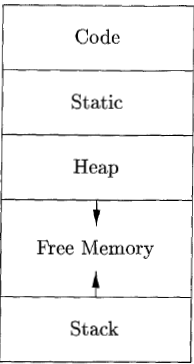
\includegraphics[scale=.4]{wk51}}
				\caption{Typical subdivision of run-time memory into code and data areas}
				\label{wk51}
			\end{figure}
		\end{center}
	\end{column}
\end{columns}
	
\end{frame}
\section{Results Obtained}
\begin{frame}{Results Obtained}
	content...
\end{frame}
\section{References}
\begin{frame}[allowframebreaks]{References}
	\bibliographystyle {abbrv}
	\bibliography {cite}
\end{frame}

\end{document}